\section{Analysis}
\label{sec:analysis}

\subsection{Property distributions}
Here we will look at the frequency distributions (histograms) comparing the characteristics of CPSBs, RPSBs an their control galaxies.

We compare the distributions of CPSBs with that of the RPSB sample in terms of S\'ersic index, stellar mass, and redshift. These distributions are taken from the data in Tables \ref{tab:my-CPSBs} and \ref{tab:my-RPSBs}. The frequency distribution histograms are plotted in Figures \ref{fig:Sersic-plot}, \ref{fig:stellar-mass-plot} and \ref{fig:redshift-plot} respectively.

\begin{figure}
    \centering
    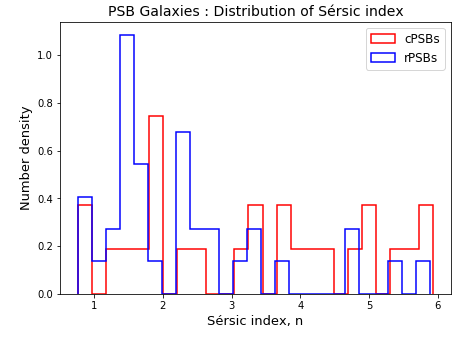
\includegraphics[width=\columnwidth]{images/JupyterPlots/Seric-index-distribution.png}
    \caption{Distribution of S\'ersic index values.}
    \label{fig:Sersic-plot}
\end{figure}

\begin{figure}
    \centering
    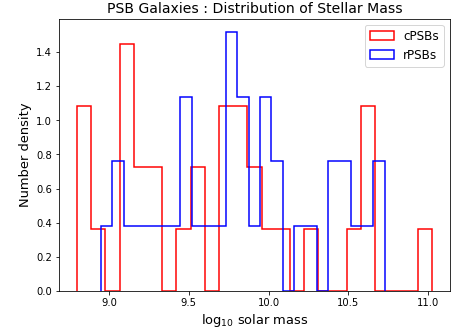
\includegraphics[width=\columnwidth]{images/JupyterPlots/Stellar-mass-distribution.png}
    \caption{Distribution of Stellar mass.}
    \label{fig:stellar-mass-plot}
\end{figure}

\begin{figure}
    \centering
    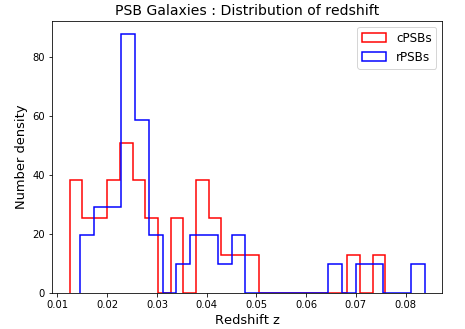
\includegraphics[width=\columnwidth]{images/JupyterPlots/Redshift-distribution.png}
    \caption{Distribution in redshift.}
    \label{fig:redshift-plot}
\end{figure}

\begin{figure}
    \centering
    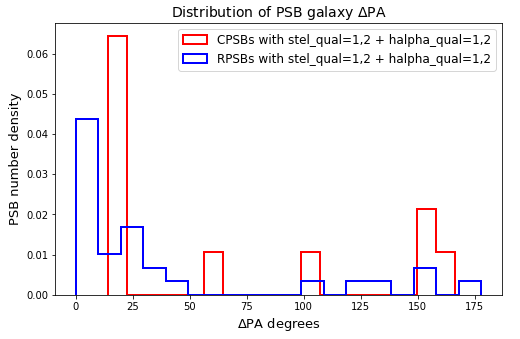
\includegraphics[width=\columnwidth]{images/JupyterPlots/Distribution-of-PSB-deltaPA.png}
    \caption{Distribution of PSB galaxy velocity map position angles.}
    \label{fig:deltaPAdistribution}
\end{figure}

We now look at the velocity map position angle variance in the control galaxies as shown in Figure \ref{fig:controlDeltaPAs}.

\begin{figure}
    \centering
    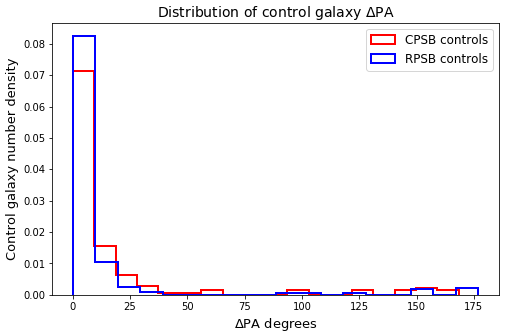
\includegraphics[width=\columnwidth]{images/JupyterPlots/Distribution-of-control-galaxy-deltaPA.png}
    \caption{Distribution of control galaxy velocity map $\Delta$PA.}
    \label{fig:controlDeltaPAs}
\end{figure}

\begin{figure}
    \centering
    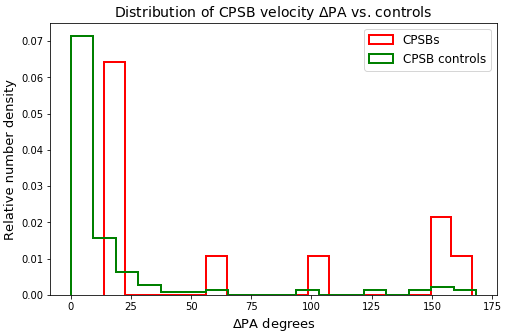
\includegraphics[width=\columnwidth]{images/JupyterPlots/Distribution-of-CPSB-dPA-vs-controls.png}
    \caption{Distribution of CPSB stellar-gas velocity $\Delta$PA vs. controls.}
    \label{fig:CPSBvsControlDeltaPAs}
\end{figure}

\begin{figure}
    \centering
    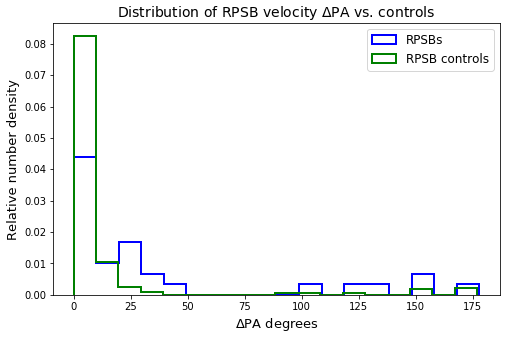
\includegraphics[width=\columnwidth]{images/JupyterPlots/Distribution-of-RPSB-dPA-vs-controls.png}
    \caption{Distribution of RPSB stellar-gas velocity $\Delta$PA vs. controls.}
    \label{fig:RPSBvsControlDeltaPAs}
\end{figure}


